%%%%%%%%%%%%%%%%%%%%%%%%%%%%%%%%%%%%%%%%%%%%%%%%%%
%  JASA LaTeX Template File
%  To make articles using JASA.cls, Version 1.1
%  September 14, 2019
%%%%%%%%%%%%%%%%%%%%%%%%%%%%%%%%%%%%%%%%%%%%%%%%%%

%% Step 1:
%% Uncomment the style that you want to use:

%%%%%%% For Preprint
%% For manuscript, 12pt, one column style

%% Comment this out if you'd rather use another style:
\documentclass[preprint]{JASA}
%\usepackage{makecell}
%\usepackage{multirow}
\usepackage[T1]{tipa}
%\usepackage{hyperref} % for urls
\usepackage{rotating} % to rotate images

%%%%% Preprint Options %%%%%
%% The track changes option allows you to mark changes
%% and will produce a list of changes, their line number
%% and page number at the end of the article.
%\documentclass[preprint,trackchanges]{JASA}


%% NumberedRefs is used for numbered bibliography and citations.
%% Default is Author-Year style.
%% \documentclass[preprint,NumberedRefs]{JASA}

%%%%%%% For Reprint
%% For appearance of finished article; 2 columns, 10 pt fonts

% \documentclass[reprint]{JASA}

%%%%% Reprint Options %%%%%

%% For testing to see if author has exceeded page length request, use 12pt option
%\documentclass[reprint,12pt]{JASA}


%% NumberedRefs is used for numbered bibliography and citations.
%% Default is Author-Year style.
% \documentclass[reprint,NumberedRefs]{JASA}

%% TurnOnLineNumbers
%% Make lines be numbered in reprint style:
% \documentclass[reprint,TurnOnLineNumbers]{JASA}
%\usepackage{algpseudocode}

\begin{document}

%% the square bracket argument will send term to running head in
%% preprint, or running foot in reprint style.


\title{Perceptual normalization for speaking rate occurs below the level of the syllable \thanks{This work was supported by National Institute on Deafness and Other Communication Disorders grants T32DC000046 and F32DC019539 (M.C.) and 5R01HD081127 (R.S.N.).}}

\author{Margaret Cychosz}
\author{Rochelle S. Newman}
\affiliation{Department of Hearing and Speech Sciences, University of Maryland, College Park, College Park, MD}


\begin{abstract} 
Because speaking rates are highly variable, listeners must use cues like phoneme or sentence duration to normalize speech across different contexts. Scaling speech perception in this way allows listeners to distinguish between temporal contrasts, like voiced and voiceless stops, even at different speech speeds. It has long been assumed that this speaking rate normalization can occur over small units such as phonemes. However, phonemes lack clear boundaries in running speech, so it is not clear that listeners can rely on them for normalization. To evaluate this, we isolate two potential processing levels for speaking rate normalization---syllabic and sub-syllabic---by manipulating phoneme duration in order to cue speaking rate, while also holding syllable duration constant. In doing so, we show that changing the duration of phonemes both with unique spectro-temporal signatures (/k\textscripta/) and more overlapping spectro-temporal signatures (/w\textsci/) results in a speaking rate normalization effect. These results suggest that when acoustic boundaries within syllables are less clear, listeners can normalize for rate differences on the basis of sub-syllabic units.

\end{abstract}

\maketitle


\section{Introduction}\label{intro}

Speaking rate varies widely between and within speakers. Yet many phonological contrasts of the world's languages rely on temporal cues, such as vowel length or voice onset time (VOT), whose raw values vary by speech rate. Consequently, listeners must perceptually \textit{normalize} for speaking rate, remapping acoustic cues across different contexts and speakers, in order to comprehend speech and acquire language. 

Listeners employ perceptual normalization (or compensation) for speaking rate over a variety of levels in the speech signal.\footnote{Throughout the paper, we refer to normalization for speaking rate without implying that listeners normalize for all contextual information during perception. We also do not use the term ``normalization'' to imply that listeners eliminate vs. maintain rate-based information.} For example, to categorize a temporally-cued contrast like /k-g/, listeners could use \textit{proximal} information in the speech signal, like the duration of vowels or consonants that are adjacent to the target phoneme 
\citep{diehlAuditoryBasisStimulus1989,millerEffectsLateroccurringInformation1979,newmanPerceptualNormalizationSpeaking1996,summerfieldArticulatoryRatePerceptual1981}. Listeners could also use \textit{distal} information in the speech signal like the rate of the overall sentential context, another talker's habitual or situational speaking rate, or even the duration of non-speech stimuli like tones \citep{maslowskiHowTrackingHabitual2019, newmanPerceptualNormalizationSpeaking2009,reinischSpeakerspecificProcessingLocal2016,wadePerceptualEffectsPreceding2005}. In both cases, for a contrast like /k-g/, shorter-duration cues (e.g., a shorter adjacent consonant or a faster sentence) suggest a faster speaking rate and therefore bias listeners to the positive VOT phoneme /k/. In contrast, longer-duration cues bias listeners to the negative or neutral VOT phoneme /g/. 

Research on proximal information for speaking rate normalization has focused on cues such as the duration of phones preceding or following the target segment. As a result, we now know that although there are more degrees of freedom in vowel than consonant duration \citep{crystalSegmentalDurationsConnected1988}, both vowels and consonants can provide rate normalization cues (\citealt{diehlAuditoryBasisStimulus1989,summerfieldArticulatoryRatePerceptual1981}; see \citealt{toscanoCueintegrationContextEffects2012} for an alternative interpretation). There is evidence both for long-term, distal cues being employed during speaking rate normalization \citep{baese-berkLongtermTemporalTracking2014,maslowskiHowTrackingHabitual2019,reinischSpeakingRateProximal2011,kosemNeuralEntrainmentDetermines2018}, as well as adjacency biases as listeners normalize over limited temporal windows of single adjacent phonemes or syllables under typical listening conditions \citep{newmanPerceptualNormalizationSpeaking1996,sawuschPerceptualNormalizationSpeaking2000}. 

While careful experimental manipulations have led us to understand which cues listeners \textit{can} use during perceptual normalization for speaking rate, less is known about the specific units that listeners employ. This gap in our understanding of rate normalization processes is relevant for a number of reasons, theoretical and applied. Research into proximal cues for rate normalization has traditionally assumed that phonemes are the basic unit over which speaking rate can be normalized. But this assumption may be premature. For one thing, it is difficult for listeners to isolate phonemes in the comprehension of spontaneous, running speech. Articulatory undershoot and hypoarticulation compromise phonological contrasts \citep{johnsonHyperspaceEffectPhonetic1993,lindblomExplainingPhoneticVariation1990}. Coarticulation blurs acoustic boundaries between adjacent phones as speakers consistently anticipate upcoming speech sounds \citep{whalenCoarticulationLargelyPlanned1990}. The ability to resist coarticulatory pressures from adjacent phones decreases with increased lingual contact on the palate. The result is that some manners of articulation with more lingual contact, such as glides or laterals, are especially susceptible to coarticulation with adjacent phones \citep{recasensCoarticulatoryPatternsDegrees1985} and that some phonemes, particularly voiced, non-strident phonemes, are not reliably discriminable, meaning that their boundaries with adjacent sounds could be less clear. Syllables, however, are sometimes classified as relatively more temporally-based \citep{tilsenSpeechRhythmAnalysis2013} and temporal encoding is highly-discriminable even in noise \citep{giannelasamelliGapsinnoiseTestGap2008} and by young infants (6-12 months, with sensitivity increasing through middle childhood) \citep{trehubGapDetectionInfants1995}. It is therefore plausible that listeners would instead normalize speaking rates over units that variably carry stress, like syllables, or other segments with more well-defined acoustic boundaries which may not straightforwardly correspond to linguistic representations.

Rate normalization has often been considered a low-level, domain-general auditory process \citep{boskerAccountingRatedependentCategory2017,millerEffectsSpeakingRate1988}: it is involuntarily activated after milliseconds of exposure to a speech- \citep{reinischSpeakerspecificProcessingLocal2016} or non-speech-like stimulus and has been documented in non-human (avian) species \citep{welchEffectsSyllablefinalSegment2009}. However, it is also increasingly apparent that several higher-level constructs such as language experience \citep{baese-berkNonnativeSpeakersUse2016}, listener familiarity with the speaker \citep{kleinschmidtPerceptionVariableStructured2016,reinischSpeakerspecificProcessingLocal2016}, and some aspects of language-specific structure such as intonation \citep{steffmanIntonationalStructureMediates2019} also mediate rate normalization. It is thus possible that rate normalization interacts with additional higher-level units, such as the syllable, although this has not been empirically tested. 

Thus, understanding how rate normalization unfolds has clear relevance to theories of speech perception and learning. However, understanding the units used in rate normalization is also relevant for more applied, artificial intelligence applications. From a machine learning perspective, invariance in the speech signal is a central obstacle to achieving higher-performing speech-to-text and automatic speech recognition applications. Understanding appropriate mechanisms for normalization, including rate normalization, in human listeners may facilitate machine performance, as it may be simpler to program normalization on the basis of signals that \textit{tend} to be relatively more acoustically-driven (such as syllables) than those that tend to be more linguistically-driven (phonemes). If human listeners reliably normalize for speaking rate at the phonemic level, even in the absence of explicit acoustic boundaries, it would suggest that phonemic structure could be incorporated into natural language processing algorithms to benefit machines' learning of speech (though the mechanisms may vary by the type of speech, e.g., read versus spontaneous).  

\subsection{Cue integration as an alternative}

Some work on proximal cues for phoneme classification has suggested that listeners may not normalize for speaking rate via temporal cues such as syllable or VOT duration but rather \textit{integrate} acoustic cues that overlap with speaking rate to classify phonemes during real-time speech processing \citep{massaroConsonantVowelRatio1983,toscanoCueIntegrationCategories2010,toscanoCueintegrationContextEffects2012,toscanoTimecourseSpeakingRate2015}. For example, duration-dependent phonetic decisions, such as stop voicing, could be made sequentially by computing VOT and \textit{then} vowel duration (vowel duration is likewise a cue to stop voicing as the burstiness of voiceless stops can cause the the following vowel to de-voice slightly at onset, leading to shorter perceived duration \citep{allenEffectsSyllableinitialVoicing1999}, but see \citet{turkAcousticSegmentDurations2006}). Evidence from the visual world paradigm, as well as phoneme decision tasks, suggests that listeners do indeed integrate multiple phonetic cues in this way, sequentially, as they become available in the speech signal  \citep{mcmurrayTrackingTimeCourse2008,millerEffectsSpeakingRate1988,toscanoTimecourseSpeakingRate2015}. This result provides evidence against a speaking rate normalization account because such accounts would predict simultaneous integration of VOT and vowel duration. 

It was not the goal of this study to contrast cue integration and rate normalization accounts to explain proximal effects upon phonetic boundary shifts---and the results of \citet{toscanoCueintegrationContextEffects2012}, among others, do convincingly demonstrate that vowel length integration, not normalization for speaking rate, explains proximal effects upon stop voicing classifications. Nevertheless, should we find an effect of consonant duration in the current studies, we believe that this could be interpreted as rate normalization and not the more straightforward acoustic cue integration. This is because our target contrast for both studies, /\textesh-\textteshlig/, will be cued by the duration of the following \textit{consonant}, not vowel (/k/ in /\textesh k\textscripta s/-/\textteshlig k\textscripta s/ for Exp. 1 and /w/ in /\textesh w\textsci b/-/\textteshlig w\textsci b/ for Exp. 2; these stimuli will be explained in more detail in the following section). But more importantly, there is no evidence that stop or glide duration reliably indicates fricative-affricate classification. And unlike the effect of stop aspiration upon perceived vowel length (aspiration causes vowel de-voicing), there is no phonetic reason to assume that fricatives and affricates would have different effects on /k/ or /w/ duration or voicing. Consequently, should the current study find an effect of consonant duration/speaking rate upon the phonetic boundary shift between /\textesh/ and /\textteshlig/, it could indicate rate normalization, not cue integration. 

\subsection{Current study}

The present experiments were designed to investigate the effects of acoustic separability, or the ability to distinguish between two adjacent phonemes, on speaking rate normalization. Here and throughout the manuscript we will refer to ``rate normalization'' broadly, though we wish to emphasize that our results concern backward, proximal rate effects. The overarching goal is to understand the processing level (syllabic or sub-syllabic) involved in the perceptual normalization of speaking rate. In a pair of phoneme category rating experiments, we asked whether phones differing in acoustic separability (acoustically-distinct /k\textscripta/ versus overlapping /w\textsci/) would result in separate rate normalization effects or in a single combined rate normalization effect. We chose to evaluate the effects of speaking rate upon the perception of the /\textesh -\textteshlig/ contrast in American English as this contrast has demonstrated a rate normalization effect in prior research \citep{newmanPerceptualNormalizationSpeaking1996,reppPerceptualIntegrationAcoustic1978} and its primary acoustic cue is temporal. For example, \citet{reppPerceptualIntegrationAcoustic1978} manipulated the duration of noise (frication) and silence between words in the phrase ``gray ship'' and found that shorter noise intervals predisposed listeners to hear word-initial /\textteshlig/ or ``gray chip.'' Similarly, in \citet{newmanPerceptualNormalizationSpeaking1996}, the authors were able to trigger a /\textesh-\textteshlig/ phonetic boundary shift in a nonce word series ranging from /\textesh k\textscripta s/ - /\textteshlig k\textscripta s/ (``shkas'' to ``chkas'') by adjusting the duration of /k/ in the stimuli. Ambiguous stimuli, with a longer /k/ duration, suggested a slower speaking rate and biased listeners to perceive /\textteshlig/ while a shorter-duration /k/ suggested a faster speaking rate and biased listeners to perceive /\textesh/. 

A limitation of previous work on this topic, including \citet{newmanPerceptualNormalizationSpeaking1996}, is that changes to the duration of a single phoneme like /k/ also rendered changes to the duration of the surrounding syllable (e.g. /k\textscripta/) and word (e.g. /\textesh k\textscripta s/): a longer-duration /k/ resulted in a longer /k\textscripta/ syllable and /\textesh k\textscripta s/ word. As a result, any rate normalization effect could just as easily be attributed to the duration of the manipulated phoneme as the duration of the entire syllable or word.

To isolate sub-syllabic information as the potential processing unit in speaking rate normalization, Experiment 1 uses the same /\textesh k\textscripta s/-/\textteshlig k\textscripta s/ series as previous work but varies the syllable nucleus /\textscripta/ duration in the opposite direction of /k/. This manipulation leads to a /\textesh k\textscripta s/-/\textteshlig k\textscripta s/ series with consistent syllable and word, but varying phoneme, durations. Although this adjustment to the original stimuli design is small, it has important consequences: all previous work that attempted to identify the units that listeners use in rate normalization had a confound in the stimuli design and as such, to date, we have not been able to identify the units that listeners use. In the current design, any rate normalization effect cannot be due to syllable or word durations, as the series did not differ in these respects.\footnote{Although both consonant and vowel durations were manipulated, it is unlikely that an observed rate normalization effect in the expected direction would be due to manipulations to the vowel. And even if it were vowel-driven, the effect would proceed in the direction opposite to the one expected and would thus be identifiable. Such an effect would run counter to well-known observations in the literature---that shorter durations bias faster speaking rates---and would be illogical from a perceptual point of view.} Instead, the normalization effect could only be caused by variation in the manipulated phoneme /k/. Finding a rate normalization effect would suggest that the /k/ was treated as a separate unit from the following vowel and that rate normalization took place over sub-syllabic, potentially phoneme-sized, units. 

Varying the nucleus duration in the opposite direction of the consonant is unlikely to cancel out any potential effect of the consonant's duration because duration effects are (1) weighted by distance (and /k/ is linearly closer to the target contrast in the /\textesh k\textscripta s/-/\textteshlig k\textscripta s/ series) and (2) proportional (and /k/ is much shorter than /\textscripta/ so similar durational changes (e.g. 20 ms) have disproportionate impacts upon /k/ and /\textscripta/). Indeed, we do find a rate normalization effect in Experiment 1, suggesting that changing the vowel duration in the opposite direction did \textit{not} cancel out any consonant duration effect. Finding a rate normalization effect in the Experiment 1 stimuli leads us to conduct Experiment 2 where we again test for rate normalization effects but using syllables that contain less discriminable phones. We use a similar nonce word series ranging from /\textesh w\textsci b/ - /\textteshlig w\textsci b/ (``shwihb'' to ``chwihb'') where we manipulated the duration of /w/ in /w\textsci/. Although we did find an effect of /k/ duration upon perception of the initial /\textesh-\textteshlig/ contrast in Experiment 1, suggesting sub-syllabic level processing during rate normalization, we hypothesized that we may \textit{not} find this same effect of /w/ duration on the same /\textesh-\textteshlig/ contrast in Experiment 2, suggesting higher-level (syllable or word) processing for sequences with less-discriminable phones. 




\section{Experiment 1}\label{exp1}

\subsection{Methods}

\paragraph{Participants}

Twenty-one members of the University of Iowa community participated in this experiment for course credit. All listeners were native speakers of American English, and had no reported history of a speech or hearing impairment. An additional 8 listeners completed the experiment, but their data were removed because in later questioning they were found not to be a native English speaker (n=1) or they failed to respond on at least 80\% of trials (n=7) due to an automatic 3000 ms trial timeout. We cannot be sure why these participants failed to respond, but it could be due to task fatigue or boredom. The remaining participants responded to, on average 91.3\% of trials (SD=5.92). 

\paragraph{Stimuli}

An adult native English-speaking man was recorded producing the syllable /\textesh k\textscripta s/ in carrier phrases (“He said the word \textit{X}.”). His speech was digitized via a 12-bit, analog-to-digital converter at a 10-kHz sampling rate, low-pass filtered at a 4.8 kHz, and amplified. The initial consonant /\textesh/ was then separated from the remainder of the syllable, with the boundary being the onset of closure for the following /k/. A continuum of ten items, /\textesh/-/\textteshlig/, was then created by removing successive 10-ms sections from the /\textesh/ onset. A linear amplitude ramp, with duration varying along with frication duration, was used over the initial portion of each token to give the items a more natural attack. The duration of the ramp varied from 6 to 60 ms, with a 9 ms step. The resulting series ranged from 60-145 ms in duration, with the longer frication sounding more similar to a /\textesh/ and the shorter frication sounding more similar to a /\textteshlig/. Further details on the original stimulus creation can be found in \citet{newmanPerceptualNormalizationSpeaking1996}. 

The remainder of the word---the syllable /k\textscripta s/---was edited to create two new syllables, one with a shorter /k/ (and longer /\textscripta/) and one with a longer /k/ (and shorter /\textscripta/). We interpreted the /k/ to include the closure, burst, aspiration, and first four pitch pulses (which appeared to correspond to the transition of the first formant). The duration of this base /k/ was between 1/3 and 1/2 that of the vowel (see Figure \ref{fig:schema-exp1}). Thus, an equivalent amount of change in duration for /k/ and /\textscripta/ will be much larger proportionately for /k/. 

\begin{figure}
\centering
\includegraphics[scale=.75]{Figure1.pdf}
\caption{\label{fig:schema-exp1}} Speaking rate manipulations on the basis of /k/ duration and stimuli duration for first step of series: Experiment 1. 
\end{figure}

\begin{table}
\caption{\label{tab:stim-duration} Stimuli duration (ms): Experiments 1 and 2. The fricative represents the first point on the continuum (most \textesh-like).}
\centering
\begin{tabular}[t]{lllll}
Speaking rate | & \textesh & k & a & s \\
\hline
Slow & 145 & 119 & 202 & 198 \\
Base & &    98  & 223 &  \\
Fast & &    86  & 235 & \\
\hline
Speaking rate | & \textesh & w & \textsci & b \\
Slow & 102 & 62 & 151 & 174 \\
Base &  & 52 & 161 & \\
Fast &  & 35 & 178 & \\
\end{tabular}
\end{table}

The duration of /k/ was altered by removing or reduplicating pitch pulses and sections of burst and aspiration. Only short, nonadjacent sections of burst and aspiration were deleted or reduplicated so as to maintain the general amplitude profile and prevent the perception of frozen noise. No change was made to the closure duration; although closures do tend to vary slightly with speaking rate, this variability is typically quite small \citep{crystalSegmentalDurationsConnected1988,gayEffectSpeakingRate1978}, and thus unlikely to have a substantial perceptual effect. For the short /k/ stimulus, two pitch pulses were removed, as well as 17.2 ms of the burst and aspiration; for the long /k/ stimulus, four pitch pulses and 22 ms of the burst and aspiration were reduplicated. The number of pitch pulses was modeled on the number that the model speaker used when asked to speak quickly and slowly. The vowel duration was similarly adjusted by removing or reduplicating nonadjacent pitch pulses, so as to make the absolute amount of change in the vowel as close as possible to the absolute amount of change in the stop consonant. The original /k/ stimulus served as the intermediate duration stimulus resulting in a 3-way /k/-duration series (short-k/fast speaking rate, intermediate-k/base speaking rate, and long-k/slow speaking rate), although we make no claims as to the baseline item actually being half-way between the other two stimuli perceptually. The short /k/, base /k/, and long /k/ versions of the syllable were then appended to each member of the 10-item /\textesh k\textscripta s/-/\textteshlig k\textscripta s/ series. See table \ref{tab:stim-duration} for additional details. 

\paragraph{Procedure}

Participants completed 1 practice/training block of 60 trials and 4 test blocks of 90 trials each. The four 90-trial test blocks were comprised of three repetitions of each of the 30 stimuli (3 /k/ durations X 10-step /\textesh-\textteshlig/ continuum) for a total of 360 trials per participant, or 12 repetitions of each stimulus. Trials in the training block were identical to those in the test block, but comprised of two repetitions of each stimulus. Responses from the training block were not analyzed.

The stimuli were presented to listeners via a lab-created software program that randomized stimulus presentation within each block on a Macintosh 7100/AV computer. Stimuli were presented at a comfortable listening level over Audiotechnica ATH-M40 headphones. Listeners were prompted with each stimulus and asked to rate the quality of the initial phoneme on a six-point scale, ranging from ``an excellent \textit{sh}'' to ``an excellent \textit{ch}'', by pressing the appropriate button on a computer-controlled response box. Specifically, listeners were told that they should use 1 for a good, clear \textit{sh}, 2 for an okay \textit{sh}, 3 if they were guessing it was \textit{sh}, 4 if they were guessing \textit{ch}, 5 for an okay \textit{ch}, and 6 for a good, clear \textit{ch}. A label was also posted above the response box to match number to the category endpoints (`1' for excellent \textit{sh} and `6' for excellent \textit{ch}). %The use of ratings allowed the detection of subtle differences within a category that may not have been obvious with simpler, categorical labeling \citep{sawuschSelectiveAdaptationEffects1976}. 
Presentation pace depended on the subject's response rate. Each trial began 1000 ms after the listener had responded to the previous trial, or after an interval of 3000 ms following stimulus onset, whichever came first. The experiment lasted approximately 45 minutes. 

\subsection{Results}

Data were analyzed in the RStudio computing environment (version: 1.4.1103; \citealt{rstudioteamRStudioIntegratedDevelopment2020}). Visualizations were created with \texttt{ggplot2} \citep{wickhamGgplot2ElegantGraphics2016}. Modeling was conducted and presented using the \texttt{lme4} \citep{batesFittingLinearMixedeffects2015}, \texttt{lmerTest} \citep{kuznetsovaLmerTestPackageTests2017}, and \texttt{broom.mixed} \citep{bolkerBroomMixedTidying2020} packages. Data analysis decisions (modeling) were not formally pre-registered, but were planned prior to data viewing and are thus confirmatory and not exploratory. Code to replicate these analyses is available in the project's GitHub respository (\url{https://github.com/megseekosh/rate-normalization}). 

To illustrate a possible effect of phoneme duration on rate normalization, we first visualize (1) the proportion of /\textesh/ responses and (2) overall /\textesh/-ness ratings. For the proportion of /\textesh/ responses, the summed proportion of ``1'', ``2'', and ``3'' responses (indicating better /\textesh/) were calculated for each participant, for each stimulus item, by dividing the number of ``1-3'' ratings by all ratings for a given participant/stimulus (Figure \ref{fig:exp1-response-function}A). /\textesh/-ness ratings were simply computed for each individual stimulus item presented (item-level) (Figure \ref{fig:exp1-response-function}B. Overall /\textesh/-ness ratings are only plotted for illustration; statistical modeling was performed on binomial /\textesh/ responses, so effects are reported in log odds. %We elected to model two outcomes because traditional work on rate normalization has modeled percentage phoneme responses grouped over stimuli repetitions (e.g. \citealt{diehlAuditoryBasisStimulus1989}), while newer work has been able to model item-level effects (e.g. \citealt{maslowskiHowTrackingHabitual2019}) and we wished to make our work comparable to both of these domains.

%\begin{sidewaysfigure}
\begin{figure}
\centering
\includegraphics[scale=.8]{Figure2.pdf}
\caption{\label{fig:exp1-response-function} A: Spaghetti plot of percentage /\textesh/ response by series step and speaking rate: /k/ duration manipulation. B: Spaghetti plot of /\textesh/-ness ratings (1=good /\textesh/, 6=good /\textteshlig/) by series step and speaking rate: /k/ duration manipulation. Both: Thick, color lines represent group averages by speaking rate and lighter lines represent individual participant responses. Ribbons represent 95\% confidence intervals.}
\end{figure}
%\end{sidewaysfigure}

Figures \ref{fig:exp1-response-function}A and \ref{fig:exp1-response-function}B suggest that the presence of a rate normalization effect from phoneme duration manipulations. The confidence intervals surrounding the speaking rate conditions (Slow, Base, Fast) do not overlap in the middle, ambiguous section of the continuum. More specifically, we see the effect in the expected direction: slower speaking rates bias /\textteshlig/ responses and higher /\textteshlig/ ratings, while faster rates bias /\textesh/ responses and higher /\textesh/ ratings.

%\begin{figure}
%\centering
%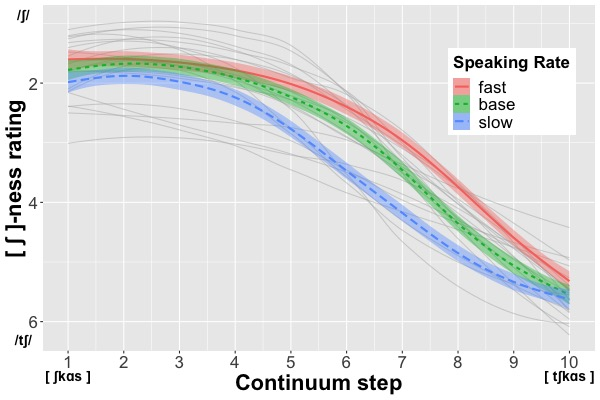
\includegraphics[scale=.5]{exp1-eshness-rating.jpeg}
%\caption{\label{fig:exp1-eshness-rating} Spaghetti plot of /\textesh/-ness ratings (1=good /\textesh/, 6=good /\textteshlig/) by series step and speaking rate: /k/ duration manipulation. Thick, color lines represent group averages by speaking rate and lighter lines represent individual participant responses. Ribbons represent 95\% confidence intervals.}
%\end{figure}

To examine a potential rate normalization effect, we fit a mixed effects model with a logistic linking function to predict the log-odds of a /\textesh/ response. This logistic function accounts for the binomially distributed categorical outcome variable \citep{queneExamplesMixedeffectsModeling2008}. Ratings of 1-3 indicate an /\textesh/-bias response and 4-6 indicate /\textteshlig/-bias response, in line with the instructions that participants received when completing the task. The dependent variable was subsequently re-coded to /\textesh/=1 and /\textteshlig/=0, so positive model coefficients in the summary indicate more /\textesh/ responses. The maximal random effects structure was fit and then backwards pruned until the model converged \citep{barrRandomEffectsStructure2013}. Backwards pruning began by eliminating correlations and then slopes, preferencing the removal of random effects with the smallest variance. Fixed effects were added step-wise, though we additionally evaluated fixed effects via backward fitting and concluded with the same models; this is explained in further detail below. Model parameter significance was determined via a combination of likelihood ratio tests between models, AIC estimations, and p-values (under $\alpha$ <.05 criterion) from model summaries.

The final random effect-only model included Participant-level intercepts; random slopes of Speaking Rate and Continuum Step by Participant, as well as Speaking Rate by Continuum Step, did not converge and were removed from the maximal random effect-only model. The fixed effect of Speaking Rate (modeled categorically with simple coding ``Slow,'' ``Base,''\textsubscript{(reference)} and ``Fast'') improved upon the random effects-only model as did Continuum Step (modeled as a continuous variable and centered at 0 by subtracting the mean) (Table \ref{tab:exp1-sh-prop-model-summary}). The interaction of Continuum Step and Speaking Rate did not improve upon a model where these parameters were modeled independently.

Unsurprisingly, the proportion of /\textesh/ responses decreased with increased steps along the /\textesh/-/\textteshlig/ continuum (\(\beta\)=-0.74, z=-43.14, p\textless.001). For Speaking Rate, there was a greater proportion of /\textesh/ responses in the Fast condition than the Base condition (\(\beta\)=0.53, z=6.24, p\textless.001) and a lower percentage of /\textesh/ responses in the Slow condition than Base (\(\beta\)=-0.81, z=-9.57, p\textless.001), suggesting a rate normalization effect.

\begin{table}
\caption{\label{tab:exp1-sh-prop-model-summary}Model predicting /\textesh/ responses: Experiment 1}
\centering
\begin{tabular}[t]{cccccc}
\toprule
Parameter & Estimate & S.E. & z-statistic & p-value & 95\% CI\\
%\midrule
Intercept & 0.85 & 0.14 & 6.00 & p\textless.001 & 0.58 – 1.13\\
Rate:Fast & 0.53 & 0.09 & 6.24 & p\textless.001 & 0.36 – 0.7\\
Rate:Slow & -0.81 & 0.08 & -9.57 & p\textless.001 & -0.98 – -0.64\\
Continuum Step & -0.74 & 0.02 & -43.14 & p\textless.001 & -0.77 – -0.71\\
%\bottomrule
\end{tabular}
\end{table}


%. The random effect structure again included the maximal number of terms that permitted model convergence, in this case random effects of Participant and Item. There were significant main effects of Continuum Step and Speaking Rate (Table \ref{tab:exp1-sh-rating-model-summary}). Ratings increased with continuum steps, indicating increased perception of /\textteshlig/ (\(\beta\)=0.50, z=10.79, p<.001). Most importantly, the Slow speaking rate condition predicted higher ratings, or more /\textteshlig/-ness, than the Base speaking rate condition (\(\beta\)=0.59, z=4.67, p=.005): a longer /k/ duration, suggesting a slower speaking rate, biased listeners to perceive and rate the stimuli as more /\textteshlig/-like. However, there was only a reliable effect of Speaking Rate in the Slow condition; the difference between the Fast and Base speaking rates upon listeners' rankings approached but did not reach significance.

%\begin{table}
%\caption{\label{tab:exp1-sh-rating-model-summary}Model predicting /\textesh/-ness ratings: Experiment 1. Lower value indicates more /\textesh/-like.}
%\centering
%\begin{tabular}[t]{lrrrrl}
%\hline\noalign{\smallskip}
%Parameter & Estimate & S.E. & z-statistic & p-value & 95\% CI\\
%\hline\noalign{\smallskip}
%Intercept & 1.31 & 0.18 & 7.16 & <.001 & 0.95 - 1.66 \\
%Rate:Fast & -0.27 & 0.13 & -2.14 & 0.052 & -0.52 - -0.02 \\
%Rate:Slow & 0.59 & 0.13 & 4.67 & 0.005 & 0.34 - 0.84 \\
%Continuum Step & 0.50 & 0.05 & 10.79 & <.001 & 0.41 - 0.59 \\
%\hline\noalign{\smallskip}
%\end{tabular}
%\end{table}


Overall, these results demonstrate that manipulating /k/ duration, while holding the syllable duration constant, significantly affected the proportion of /\textesh/ responses, suggesting that listeners can normalize for speaking rate over sub-syllabic units such as phonemes.

\subsection{Interim discussion}

Experiment 1 demonstrated that two phonemes with obvious acoustic boundaries, /k/ and /\textscripta/, were treated as separate units during rate normalization. This result implies that the processing unit during rate normalization is something smaller than a syllable. However, /k/ and /\textscripta/ are fairly acoustically distinct and separable during running speech. It could be that listeners only rely on sub-syllabic structure to normalize for speaking rate when syllables have a well-defined internal structure. Do listeners likewise normalize for speaking rate over sub-syllabic units that are more difficult to distinguish? 

Experiment 2 examines a syllable containing phonemes that are much more difficult to segment acoustically: a glide and a vowel. To examine this, we chose a nonce word series that ranged from /\textesh w\textsci b/-/\textteshlig w\textsci b/. Previous work on similar stimuli---a /sw\ae b/-/tw\ae b/ continuum---demonstrated that varying the /w/ duration while leaving the vowel constant, and varying the /\ae/ duration while leaving the glide constant, both lead to a change in category boundary location for the initial /s-t/ contrast \citep{newmanPerceptualNormalizationSpeaking1996}. Yet, as outlined in the justification for experiment 1, this effect could have been driven by the duration of a unit larger than the phoneme, because changing the /w/ duration while leaving the /\ae/ constant results in the combined syllabic unit also being longer. Consequently, as in Experiment 1, we again varied the /w/ duration while also altering the /\textsci/ duration in the opposite direction, leading to a series with consistent syllable and word durations. If /w/ and /\textsci/ are treated as separate units during rate normalization like /k/ and /\textscripta/ were, despite the acoustic inseparability between /w/ and /\textsci/, then manipulating the duration of /w/ should lead to a rate normalization effect in this series. 

\section{Experiment 2}\label{exp2}

\subsection{Methods}

\paragraph{Participants}

Twenty-two members of the University of Iowa community participated in this experiment for course credit. All were native English speakers with no reported history of a speech or hearing impairment and had not participated in experiment 1. Three participants did not respond on at least 80\% of the trials, so their data were removed from analysis leaving 19 participants. The remaining participants responded to, on average 92.78\% of trials (SD=5.18). 

\paragraph{Stimuli}

Stimulus creation was nearly identical to that in Experiment 1. The same speaker produced the syllable /\textesh w\textsci b/ in the same manner previously described. The initial fricative was separated from the remainder of the syllable, with the boundary being the zero-crossing preceding the first pitch pulse of the /w/. A series of ten items ranging from /\textesh/ to /\textteshlig/ was created in a similar manner as Experiment 1, by removing successive sections of approximately 10 ms from the onset of the /\textesh/. 

The syllable /w\textsci/ was edited in the same manner as the /k\textscripta/ syllable in Experiment 1. Based on spectral analysis, the first 7 vocal pulses were considered part of /w/ rather than the /\textsci/, because these pulses appeared to constitute the /w/ formant transitions (especially those of the first formant). We lengthened and shortened the /w/ and /\textsci/ durations by reduplicating or deleting nonadjacent pitch pulses in the same manner as before, again modeled on the number that the speaker used when asked to speak quickly and slowly. For the shorter /w/, three pitch pulses were removed, whereas four pulses were reduplicated to create the long /w/ (and pitch pules from the vowel were likewise removed or reduplicated in the same manner to keep the syllable duration constant). The original items served as the intermediate duration. The /w/ duration was shorter than that of the /\textsci/, so the same amount of absolute change resulted in a larger change proportionately for the /w/ than for the vowel. The short /w/, baseline /w/, and long /w/ versions of the syllable were then appended to each member of the 10-item /\textesh/-/\textteshlig/ series. This resulted in three /w/-duration series with a constant syllable and word duration, but varying /w/ (and vowel) durations.

\begin{figure}
\centering
\includegraphics[scale=.75]{Figure3.pdf}
\caption{\label{fig:schema}} Speaking rate manipulations on the basis of /w/ duration and stimuli duration for first step of series: Experiment 2. 
\end{figure}

\paragraph{Procedure}

The procedure was identical to that of Experiment 1.

\subsection{Results}

As in experiment 1, the percentage of /\textesh/ response was calculated for each participant (Figure \ref{fig:exp2-response-function}A) and /\textesh/-ness ratings were computed for each individual stimulus item (Figure \ref{fig:exp2-response-function}B). The visualizations suggest an effect of speaking rate (/w/ duration) upon /\textesh/ responses and /\textesh/ ratings in the same direction as Experiment 1: slower speaking rates bias more /\textteshlig/ responses.

%\begin{sidewaysfigure}[htpb]
\begin{figure}
\centering
\includegraphics[scale=.75]{Figure4.pdf}
\caption{\label{fig:exp2-response-function}A: Spaghetti plot of percentage /\textesh/ response by series step and speaking rate: /w/ duration manipulation. B: Spaghetti plot of /\textesh/-ness ratings (1=good /\textesh/, 6=good /\textteshlig/) by series step and speaking rate: /w/ duration manipulation. Both: Thick, color lines represent group averages by speaking rate and lighter lines represent individual participant responses. Ribbons represent 95\% confidence intervals.}
\end{figure}
%\end{sidewaysfigure}

For the modeling, to evaluate a potential rate normalization effect, we again fit a mixed effects model with a logistic linking function to predict /\textesh/ responses. All variables were coded as an Experiment 1. The model fitting procedure was likewise the same. The final random effect-only model only included intercepts for Participant; more complex random effects structures did not converge. Both the fixed effects of Speaking Rate and Continuum Step, but not their interaction, improved upon a model fit (as in experiment 1). See Table \ref{tab:exp2-sh-prop-model-summary} for summary.

%\begin{figure}
%\centering
%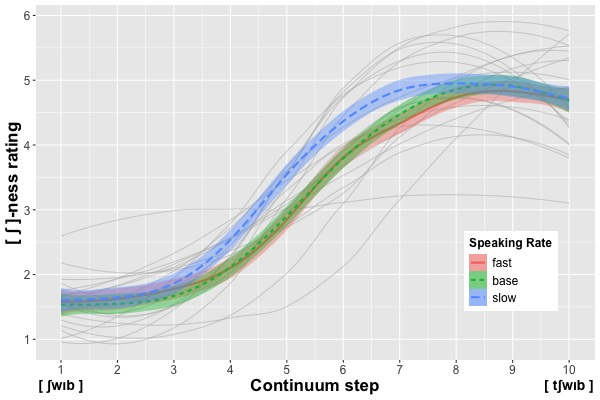
\includegraphics[scale=.5]{exp2-eshness-rating.jpeg}
%\caption{\label{fig:exp2-eshness-rating}Spaghetti plot of /\textesh/-ness ratings (1=good /\textesh/, 6=good /\textteshlig/) by series step and speaking rate: /w/ duration manipulation. Thick, color lines represent group averages by speaking rate and lighter lines represent individual participant responses. Ribbons represent 95\% confidence intervals.}
%\end{figure}


\begin{table}

\caption{\label{tab:exp2-sh-prop-model-summary}Model predicting /\textesh/ responses: Experiment 2}
\centering
\begin{tabular}[t]{cccccc}
\toprule
Parameter & Estimate & S.E. & z-statistic & p-value & 95\% CI\\
%\midrule
Intercept & 0.11 & 0.13 & 0.85 & 0.40 & -0.15 - 0.38\\
Rate:Fast & 0.05 & 0.09 & 0.52 & 0.61 & -0.13 - 0.22\\
Rate:Slow & -0.43 & 0.09 & -4.86 & p\textless.001 & -0.6 - -0.26\\
Continuum Step & -0.77 & 0.02 & -42.94 & p\textless.001 & -0.8 - -0.73\\
%\bottomrule
\end{tabular}
\end{table}

Once again, unsurprisingly, the proportion of /\textesh/ responses decreased with increased steps along the /\textesh/-/\textteshlig/ continuum (\(\beta\)=-0.77, z=-42.94, p\textless.001). For Speaking Rate, there were fewer /\textesh/ responses in the Slow condition than Base, (\(\beta\)=-0.43, z=-4.86, p\textless.001), suggesting a rate normalization effect in that direction. However, there were no reliable differences in /\textesh/ responses between the Fast and Base speaking rate conditions. Consequently, the results from Experiment 2 show an effect of speaking rate (/w/ duration) upon the perceived phonetic boundary between /\textesh/ and /\textteshlig/ for \textit{slow} speaking rates, but not fast, indicating that normalization can occur over phonemes in sequences without clear acoustic boundaries (/w\textsci/), but perhaps only when the speaking rate is slow enough to delineate the the units. 

%Finally, we fit a model to predict /\textesh/-ness ratings for these stimuli, where a lower rating indicated that listeners considered the stimuli more /\textesh/-like. The random effect structure again included random intercepts by Participant and Item and there were significant main effects of Continuum Step and Speaking Rate (Table \ref{tab:exp2-sh-ness-model-summary}). Unsurprisingly, stimuli further along the /\textesh-\textteshlig/ continuum were perceived as more /\textteshlig/-like (\(\beta\)=0.82, z=17.66, p\textless.001). Longer /w/ durations, indicating a slower speaking rate, also biased listeners to perceive the stimuli as more /\textteshlig/-like (\(\beta\)=0.54, z=4.20, p=.003). As with Experiment 1, we did not find an effect of speaking rate in the Fast speaking rate condition. Overall, the results from Experiment 2 show an effect of speaking rate (/w/ duration) upon the perceived phonetic boundary between /\textesh/ and /\textteshlig/, indicating that normalization can occur over these phonemes without clear acoustic boundaries.

%\begin{table}
%\caption{\label{tab:exp2-sh-ness-model-summary}Model predicting /\textesh/-ness ratings: Experiment 2}
%\centering
%\begin{tabular}[t]{lrrrrl}
%\hline\noalign{\smallskip}
%Parameter & Estimate & S.E. & z-statistic & p-value & 95\% CI\\
%\noalign{\smallskip}\hline\noalign{\smallskip}
%Intercept & -1.19 & 0.30 & -3.99 & 0.002 & -1.78 - -0.61\\
%Rate:Fast & -0.06 & 0.13 & -0.49 & 0.64 & -0.31 - 0.19\\
%Rate:Slow & 0.54 & 0.13 & 4.20 & 0.003 & 0.29 - 0.79\\
%Continuum Step & 0.82 & 0.05 & 17.66 & <.001 & 0.73 - 0.91\\
%\noalign{\smallskip}\hline
%\end{tabular}
%\end{table}


\section{General discussion}

To comprehend speech and language, listeners must compensate for variation across different speakers, in different contexts. Normalization for speaking rate is one important example of this process: it allows listeners to maintain temporal contrasts, such as VOT or vowel length, across different speech speeds and between different speakers. In a pair of experiments, we evaluated whether listeners could use information from sub-syllabic units like phonemes---which coarticulation and hypoarticulation often render undefined in the acoustic signal---instead of syllables to normalize for speaking rate (backwards, and proximally). Listeners did normalize over phonemes, including acoustically-overlapping phonemes, to factor out speaking rate, demonstrating that sub-syllabic information is used during rate normalization processes.

Work on proximal information in the speech signal for rate normalization has long argued that normalization occurs over individual phones \citep{diehlAuditoryBasisStimulus1989,newmanPerceptualNormalizationSpeaking1996}. Empirical support was lacking, however, because previous work altered the duration of the carrier syllable and word in addition to the phone. Here we compensated for changes in consonant duration by also changing the nucleus duration. This step allowed us to maintain a consistent syllable duration, avoid the previous experimental confound, and isolate effects of sub-syllabic information on rate normalization. Since we replicated previous work in finding an effect of phoneme duration on this phonetic boundary shift, we can now more definitively say that listeners can use units below the level of the syllable, such as phonemes, to compute speaking rate during online speech processing. Furthermore, by also evaluating the effects of acoustic distinctiveness on rate normalization, we were additionally able to show that this phoneme processing for rate normalization even occurs in sequences like /w\textsci/ that share several acoustic features (periodicity, dynamicity, continuous dynamic formant structure) and are thus less separable. As such, this work expands upon \citet{newmanPerceptualNormalizationSpeaking1996} because the vowel was co-varied in this study and it was manipulated to a much smaller extent ([52 to 197ms] in \citet{newmanPerceptualNormalizationSpeaking1996} versus [202 to 235ms] in the current study), making it all the more interesting that a rate effect was still found. 

Rate normalization can be activated after just milliseconds of exposure \citep{reinischSpeakerspecificProcessingLocal2016}, and is documented in human and non-human species alike \citep{welchEffectsSyllablefinalSegment2009}, suggesting that this type of normalization is a low-level auditory process that could be partially domain-general. Finding that listeners can compute speaking rate over sub-syllabic units such as phonemes speaks directly to this idea. Phonemes do not relay a clear acoustic signal. They are indistinct, coarticulated, and reduced---traits that are exacerbated when the features (voicing, stridency) of adjacent phones overlap within syllables. If rate normalization were exclusively or primarily domain-general, it is unclear how listeners could normalize over individual phonemes. It is possible that listeners may \textit{prefer} or \textit{tend} to normalize over syllables, or relatively more acoustically-reliable components of speech such as word boundaries, but will compute over phonemes in the absence of higher-level information. Our experiments were not designed to contrast listeners' preferred processing unit for rate normalization. It is also possible, as \citet{boskerAccountingRatedependentCategory2017} suggests, that perceptual normalization for speaking rate could be domain general for some lower-level constructs, such as phonetic boundary shifts, but increasingly language-specific at higher levels such as determining the presence of function words \citep{dilleyAlteringContextSpeech2010}. Nevertheless, the fact that listeners could normalize over sub-syllabic information in these experiments suggests that rate normalization processes may be driven by some language-particular experience, instead of the raw acoustic signal alone. 

Although these results suggest the primacy of sub-syllabic information, such as phonemes, for rate normalization, an alternative interpretation could be that in the presence of ambiguous stimuli, listeners simply weigh information that is immediately available in the signal more than distal, high-level information. (Or that, given that the syllable duration is constant, listeners weigh longer consonants relative to shorter vowels or vice versa.) This interpretation does not require the phoneme to be a perceptual unit. Furthermore, although the current study manipulated phoneme duration, the experimental design still does not disassociate phonemes from other sub-syllabic entities for normalization, such as the duration of diphthongs or phonetic cues like formant transitions. It could be that listeners are attuned to information at ambiguous points in the signal---wherever that point of ambiguity lies. In the current studies, the ambiguous point was a phoneme boundary but future work may be able to manipulate ambiguity within a single phoneme and elicit a similar normalization effect. 

Finally, there is an interesting asymmetry in the results whereby listeners in experiment 1 used sub-syllabic information to normalize for speaking rate in all speaking rate conditions but listeners in experiment 2 only used this information to normalize in the slow speaking rate conditions. Consequently, it could be that, for less-discriminable syllables, listeners can use sub-syllabic information in slower speaking rates, but not faster because faster speech renders the phonemes too indiscriminable in sequences such as /w\textsci/. Another, related topic, could be to compare how normalization unfolds in different phonotactic sequences. Stimuli in these studies were phonotactically illicit in American English---listeners were unaccustomed to hearing onset clusters such as /\textteshlig k/ and /\textesh k/. However, it is possible that the default processing strategy during rate normalization could change based on the listener's history with a particular sequence. Perhaps rate normalization occurs more globally, at the lexical or supra-syllabic level, for sequences with high phonotactic probability but more locally at the sub-syllabic level for sequences with lower phonotactic probability. If processing strategies for rate normalization do vary by listener experience, this would be one reason to study the emergence of rate normalization skills in infants---especially given that infants as young as two months are sensitive to duration manipulations (formant transitions) \citep{eimasContextualEffectsInfant1980}---and older children where we may see changes in the default processing strategy changing as a function of child age, vocabulary size, or phonological neighborhood composition.  

The results of these experiments open up several avenues for future research. First, these experiments only tested American English listeners listening to mostly singleton consonants and monophthongal vowels embedded in nonce words. But other works have found clear effects of language structure and experience on rate normalization \citep{baese-berkNonnativeSpeakersUse2016,steffmanIntonationalStructureMediates2019}. Do listeners also normalize over units, like morae, geminates, or diphthongs that are heavier/larger than phonemes but smaller than syllables? As suggested previously, phonotactic structure is another unexplored aspect of language structure that may be relevant for understanding how listeners calculate speaking rate. Some languages, such as Japanese, tend to have more acoustically ``confusable'' internal syllable structures, only permitting nasal consonants, and not stops, in coda position for example. This element of Japanese phonotactics renders the transition between nuclei and codas less discriminable, given the shared acoustic properties of nasals and vowels, than in a language like English where a much wider array of codas are permitted (e.g. /s/, /t/). Consequently, if, as in Japanese, the acoustic signature within syllables tends to be more indistinct, listeners could, over time, learn to rely less on individual phonemes for normalization. 

It will also be important for future work to evaluate processing units for normalization in faster and more naturalistic stimuli as perceptual normalization for speaking rate is likely idiosyncratic and dependent upon the context and speaker \citep{goldingerPuzzlesolvingScienceQuixotic2003}. And more naturalistic stimuli, that contain multiple, co-varying phonetic cues (i.e formant transition duration and frequency), have previously been shown to mitigate rate normalization effects \citep{shinnLimitationsContextConditioned1985}. Here we originally hypothesized that listeners would normalize over syllables or other supra-phonemic chunks because both spectral and temporal cues to phonemes become highly confusable and indistinct, especially in fast, running speech, while more global rhythmic cues to syllables may be robust in those settings. And while our experiments instead showed reliable effects of sub-syllabic duration on the phonetic boundary shift, the experimental stimuli clearly differed from what listeners would hear and process in real-world contexts. For example, even the manipulated consonant in the ``fast'' speaking rate condition in Experiment 1 was relatively slow (91 ms) compared to the word-medial stop consonants that listeners might hear in everyday conversation. The duration of the syllable stimuli was relatively long in comparison to typical speaking rates with syllable durations closer to 250-400ms. For extremely fast speech, listeners might rely less on individual phones and more on syllables or words. Faster, naturalistic speech also drives acoustic reduction and heightened coarticulation \citep{fourakisTempoStressVowel1991,gayMechanismsControlSpeech1981}. However, these acoustic cues did not necessarily accompany the stimuli employed in these experiments as we wanted to isolate the effects of speaking rate. But extreme reduction in other, more naturalistic listening conditions could lead listeners to normalize over different units. 

\section{Conclusion}

Unlike previous work studying proximal effects on rate normalization, this study manipulated speaking rate via phoneme duration while holding the duration of carrier syllables and words constant. We still demonstrated rate effects upon the phonetic boundary shift between /\textesh/ and /\textteshlig/, both for syllables containing acoustically-distinct /k\textscripta/ and -overlapping phonemes /w\textsci/. These results present evidence that listeners process speaking rate over sub-syllabic units, even in the absence of clear acoustic boundaries within syllables, suggesting roles of linguistic structure and language experience for perceptual normalization of speaking rate.  



\begin{acknowledgements}
The authors wish to thank Jessica Burnham, Jim Sawusch, and Jan Edwards for their assistance with this work. 
\end{acknowledgements}

\section*{Data availability}
Analysis scripts to replicate modeling results are included in the affiliated GitHub repository (\url{https://github.com/megseekosh/rate-normalization}.

\section*{Conflict of interest}
The authors declare that they have no conflicts of interest.


% BibTeX users please use one of
\bibliographystyle{apalike}
\bibliography{My_Library}   % name your BibTeX data base

\end{document}

